\documentclass[hidelinks,11pt]{article}
\usepackage[a4paper,width=150mm,top=30mm,bottom=35mm]{geometry}
\usepackage[utf8]{inputenc}

\usepackage{graphicx}
\graphicspath{{images/}{../images/}}

\usepackage[table]{xcolor}
\usepackage{multirow,tabularx,longtable}
\newcolumntype{Y}{>{\centering\arraybackslash}X}

%\usepackage{sectsty}
%\allsectionsfont{\nohang}

\usepackage[titletoc]{appendix}

%\usepackage{titlesec}

\usepackage[numbers]{natbib}
\renewcommand{\refname}{\large References}  % for the article class
\renewcommand{\bibname}{\large References}  % for the report or book class
\def\bibfont{\footnotesize}

% line break in bibliography urls
\usepackage{xurl}

\usepackage{caption}
%\usepackage{tocbibind}

% indent paragraphs
\usepackage{changepage}

\usepackage{mathtools}
\usepackage{amsmath}
\usepackage{amssymb}
\usepackage{amsthm}
\usepackage{color}
\usepackage{float}
\usepackage{bm}
\usepackage{multirow, makecell}
\usepackage{enumitem}
\usepackage{bold-extra}
\usepackage[mathscr]{euscript}

% matrix with labeled rows and columns
\usepackage{kbordermatrix}

\usepackage[linesnumbered,ruled,vlined]{algorithm2e}
\SetKw{Continue}{continue}
\SetKw{Input}{Input:}
\SetKw{Output}{Output:}

%\usepackage{listings}
\usepackage{pythonhighlight}


\DeclareMathOperator{\lca}{lca}
\DeclareMathOperator*{\argmax}{arg\,max}
\DeclareMathOperator*{\argmin}{arg\,min}
\definecolor{darkgrey}{rgb}{0.2,0.2,0.2}
\newcommand{\COMMANDLINE}[1]{\begingroup\par\vspace{3mm}\color{darkgrey}\begin{adjustwidth}{1cm}{1cm}\texttt{#1}\end{adjustwidth}\vspace{3mm}\endgroup}
\newcommand{\TODO}[1]{\begingroup\color{red}#1\endgroup}
\newcommand{\OLD}[1]{\begingroup\tiny   \color{green}#1\endgroup}
\newtheorem{theorem}{Theorem}
\newtheorem{lemma}[theorem]{Lemma}
\newtheorem{corollary}[theorem]{Corollary}
\newtheorem{definition}[theorem]{Definition}
\newtheorem{fact}[theorem]{Observation}
\def\arrowedvec{\mathaccent"017E}
\newcommand{\G}{\arrowedvec{G}}
\newcommand{\unrooted}[1]{\overline{#1}}  
\newcommand{\ROOT}{\circledcirc}
\newcommand{\LEAF}{\odot}
\usepackage{wasysym}
\newcommand{\SPEC}{\newmoon}
\newcommand{\HGT}{\triangle}
\newcommand{\DUPL}{\square}
\newcommand{\child}{\mathsf{child}}
\newcommand{\degree}{\mathsf{deg}}
\newcommand{\parent}{\mathsf{par}}
\newcommand{\bmr}{\mathrel{\bm{\rightarrow}}}
\newcommand{\C}[1]{\mathscr{C}_{#1}}
\newcommand{\AX}[1]{\textnormal{#1}}

% symbol for disjoint union
\makeatletter
\def\moverlay{\mathpalette\mov@rlay}
\def\mov@rlay#1#2{\leavevmode\vtop{%
		\baselineskip\z@skip \lineskiplimit-\maxdimen
		\ialign{\hfil$\m@th#1##$\hfil\cr#2\crcr}}}
\newcommand{\charfusion}[3][\mathord]{
	#1{\ifx#1\mathop\vphantom{#2}\fi
		\mathpalette\mov@rlay{#2\cr#3}
	}
	\ifx#1\mathop\expandafter\displaylimits\fi}
\makeatother
\newcommand{\cupdot}{\charfusion[\mathbin]{\cup}{\cdot}}

% Mark overfull boxes
\overfullrule=1mm

% Hyphenation and line breaks
\hyphenation{du-pli-ca-ti-on}

% contents links etc.
\usepackage{hyperref}
\hypersetup{
	colorlinks=True,
	linkcolor=blue,
	filecolor=magenta,      
	urlcolor=cyan,
	citecolor=black,
}

%\usepackage{setspace}

\begin{document}

\begin{titlepage}
	\begin{center}
		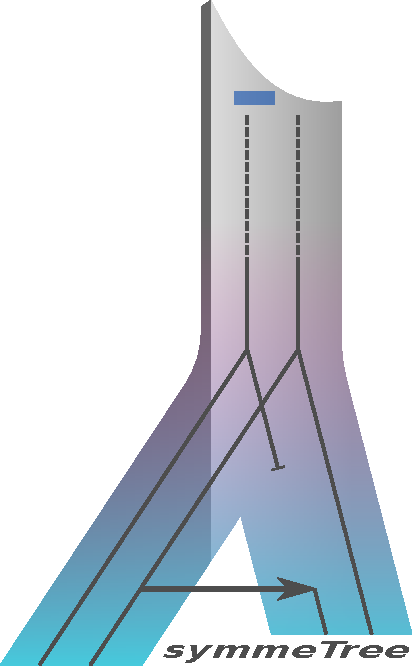
\includegraphics[width=0.4\textwidth]{logo.pdf}
	\end{center}
	\begin{center}
		\vspace*{2cm}
		
		\Huge{\fontfamily{lmtt}
			AsymmeTree User Manual
		}

		\vspace{1.5cm}
		
		\LARGE
		David Schaller\\
		\vspace{1cm}
		\large
		sdavid@bioinf.uni-leipzig.de
		
		\vspace{2cm}
		
	\end{center}
\end{titlepage}

\newpage

\tableofcontents
\newpage

\section{Introduction}

AsymmeTree is an open-source Python library for the simulation and analysis of phylogenetic scenarios.
It includes a simulator for species and gene trees with asymmetric evolution rates, tools for the inference and analysis of phylogenetic best matches \citep{geiss2019a,geiss2020c} (resp. best hits) from known gene trees or evolutionary distances. Moreover, it includes an algorithm to compute supertrees \citep{deng2016} and a method to estimate rooted species trees from an ensemble of orthology/paralogy relations \citep{hellmuth2015}.

The library, and especially the simulator, was primarily designed to be able to validate mathematical concepts and test inference methods for various steps on the way to more realistically available data, i.e., dated gene trees, additive distances of gene sets, noisy distances and finally sequences.
Both nucleotide and amino acid sequence simulation with or without indels are supported. In both cases, several substitution models are available.

The software is hosted on \href{https://github.com/david-schaller/AsymmeTree}{GitHub} and also available via The Python Package Index (\href{https://pypi.org/project/asymmetree/}{PyPI}).
Please feel free to report bugs or make suggestions for improvement in the \href{https://github.com/david-schaller/AsymmeTree/issues}{Issues} section of the GitHub repository.

If you use AsymmeTree in your project or code from it, please cite:

\vspace{3mm}
\begin{adjustwidth}{1cm}{1cm}
	Peter F. Stadler, Manuela Gei{\ss}, David Schaller, Alitzel L{\'o}pez S{\'a}nchez, Marcos Gonz{\'a}lez Laffitte, Dulce I. Valdivia, Marc Hellmuth, Maribel Hern{\'a}ndez Rosales (2020). \textbf{From pairs of most similar sequences to phylogenetic best matches.} \textit{Submitted to Algorithms for Molecular Biology.}
\end{adjustwidth}
\vspace{3mm}


\section{Installation}

AsymmeTree requires Python 3.5 or higher. Python 2 is not supported.

\subsection{Easy Installation with pip}


The \texttt{asymmetree} package is available on The Python Package Index (PyPI):

\COMMANDLINE{pip install asymmetree}

\noindent
For details about how to install Python packages see
\href{https://packaging.python.org/tutorials/installing-packages/}{here}.

\subsection{Installation with the setup file}


Alternatively, you can download or clone the repo, go to the root folder of package and install it using the command:

\COMMANDLINE{python setup.py install}


\subsection{Dependencies}

AssymmeTree has several dependencies (which are installed automatically when using \texttt{pip} or the \texttt{setup.py}):

\begin{itemize}
	\item \href{https://networkx.github.io}{NetworkX}
	\item \href{http://www.scipy.org/install.html}{SciPy and NumPy}
	\item \href{https://matplotlib.org/}{Matplotlib}
\end{itemize}

To use the tree reconstruction method for best match inference and the C++ implementation of the quartet method \citep{stadler2020}, resp., the following software must be installed
(I recommend that you compile these tools on your machine, place the binaries into a persistent location and add this location to your PATH environment variable):

\begin{itemize}
	\item \href{https://birc.au.dk/software/rapidnj/}{RapidNJ} \citep{simonsen2008}
	\item \href{https://github.com/david-schaller/qinfer}{qinfer}
\end{itemize}


\newpage

\section{Usage}

AsymmeTree is divided into several subpackages and modules, an overview of which is given in 

{\footnotesize
\setlength{\tabcolsep}{6pt}
\renewcommand{\arraystretch}{1.4}
%\renewcommand\tabularxcolumn[1]{m{#1}}
\begin{longtable}{| p{4.0cm} | p{10cm} |}
	\caption{Overview over the subpackages and modules.}\label{tab:module_overview}\\
	\endfirsthead
	\multicolumn{2}{c}{\tablename\ \thetable\ -- \textit{Continued from previous page}}\\
	\multicolumn{2}{c}{}\\
	\hline
	\endhead
	\hline \multicolumn{2}{r}{\tablename\ \thetable\ -- \textit{Continued on next page}} \\
	\endfoot
	\hline
	\endlastfoot
	%
	\hline
	%--------------------------------------------------------------------------
	\textbf{Packages and Modules} & \textbf{Description} \\
	%--------------------------------------------------------------------------
	\hline
	%--------------------------------------------------------------------------
	\multicolumn{2}{|l|}{\textbf{\texttt{treeevolve}}}\\
	%--------------------------------------------------------------------------
	\hline
	%--------------------------------------------------------------------------
	\texttt{SpeciesTree} & 
	Simulator for dated species trees with different models. \\
	%--------------------------------------------------------------------------
	\texttt{GeneTree} & 
	Simulator for dated gene trees, construction of the observable gene tree. \\
	%--------------------------------------------------------------------------
	\texttt{EvolutionRates} & 
	Simulation of evolution rate asymmetries, autocorrelation between ancestors and descendants as well as correlation between genes in the same species. \\
	%--------------------------------------------------------------------------
	\texttt{Scenario} & 
	Wrapper class for species and gene tree scenarios, computation of the (R)BMG as well as event counts and some statistics. \\
	%--------------------------------------------------------------------------
	\texttt{NoisyMatrix} & 
	Generation of a noisy matrix (random perturbation or wrong topology noise). \\
	%--------------------------------------------------------------------------
	\hline
	%--------------------------------------------------------------------------
	\multicolumn{2}{|l|}{\textbf{\texttt{tools}}}\\
	\hline
	%--------------------------------------------------------------------------
	\texttt{Tree} & 
	Includes the basic class \texttt{Tree}, provides functions for tree traversals, Newick parser, etc. \\
	%--------------------------------------------------------------------------
	\texttt{PhyloTree} & 
	Includes the class \texttt{PhyloTree} for phylogenetic trees (inherits from \texttt{Tree}), provides a Newick parser, etc. \\
	%--------------------------------------------------------------------------
	\texttt{BuildST} & 
	Includes the class \texttt{BuildST} that computes a supertree from a given list of tress (with overlapping labels) \citep{deng2016}. \\
	%--------------------------------------------------------------------------
	\texttt{DoublyLinkedList} & 
	Implementation of a doubly-linked list. \\
	%--------------------------------------------------------------------------
	\texttt{GraphTools} & 
	Miscellaneous functions for graphs such as e.g.\ check for graph equality. \\
	%--------------------------------------------------------------------------
	\hline
	%--------------------------------------------------------------------------
	\multicolumn{2}{|l|}{\textbf{\texttt{best\_matches}}}\\
	%--------------------------------------------------------------------------
	\hline
	%--------------------------------------------------------------------------
	\texttt{TrueBMG} & 
	Computation of the true (R)BMG from a gene tree as well as the true orthology relation. \\
	%--------------------------------------------------------------------------
	\texttt{ExtBestHits} & 
	Implementation of the \emph{Extended Best Hits} method, optionally uses \texttt{qinfer}. \\
	%--------------------------------------------------------------------------
	\texttt{TreeReconstruction} & 
	Reconstruction of the gene tree with \texttt{RapidNJ} \citep{simonsen2008} and midpoint rooting. \\
	%--------------------------------------------------------------------------
	\texttt{Quartets} & 
	Implementation of \emph{Quartet} approach with two different methods for outgroup selection, optionally uses \texttt{qinfer}. \\
	%--------------------------------------------------------------------------
	\texttt{LRTConstructor} & 
	Construction of a least resolved tree (LRT) from a BMG via \emph{informative triples} (optionally uses minimal edge cuts) or from a leaf-colored tree. \\
	%--------------------------------------------------------------------------
	\texttt{Augmentation} & 
	Augmentation of the least resolved tree (w.r.t.\ some BMG) in order to identify all unambiguously false orthology assignments \citep{schaller2020}. \\
	%--------------------------------------------------------------------------
	\hline
	%--------------------------------------------------------------------------
	\multicolumn{2}{|l|}{\textbf{\texttt{cograph}}}\\
	%--------------------------------------------------------------------------
	\hline
	%--------------------------------------------------------------------------
	\texttt{Cograph} & 
	Includes the classes \texttt{Cotree} and \texttt{CotreeNode} as well as a generator for random cotrees/cographs. \\
	%--------------------------------------------------------------------------
	\texttt{CographEditor} & 
	Implements a heuristic for cograph editing \citep{crespelle2019}. \\
	%--------------------------------------------------------------------------
	\texttt{LinearCographDetector} & 
	Implements an $\mathcal{O}(n+m)$ algorithm for cograph detection \citep{corneil1985}. \\
	%--------------------------------------------------------------------------
	\hline
	%--------------------------------------------------------------------------
	\multicolumn{2}{|l|}{\textbf{\texttt{paraphylo}}}\\
	%--------------------------------------------------------------------------
	\hline
	%--------------------------------------------------------------------------
	\texttt{SpeciesTreeFromParalogs} & 
	Species tree reconstruction from orthology/paralogy relations. Heuristic version of \texttt{ParaPhylo} \cite{hellmuth2015}. \\
	%--------------------------------------------------------------------------
	\texttt{SpeciesTreeFromPO} & 
	Species tree reconstruction from \texttt{ProteinOrtho} \cite{lechner2011,lechner2014} output. \\
	%--------------------------------------------------------------------------
	\hline
	%--------------------------------------------------------------------------
	\multicolumn{2}{|l|}{\textbf{\texttt{visualize}}}\\
	%--------------------------------------------------------------------------
	\hline
	%--------------------------------------------------------------------------
	\texttt{GeneTreeVis} & 
	Visualization of a (simulated) gene tree (of type \texttt{PhyloTree}), experimental. \\
	%--------------------------------------------------------------------------
\end{longtable}
}



\subsection{Tree Data Structures}

The two classes \texttt{Tree} and \texttt{PhyloTree} (inherits from \texttt{Tree}) implement tree data structures which are essential for most of the modules in the package.
The latter contains converters and parsers for the Newick format and a NetworkX graph format.

The vertices of a \texttt{PhyloTree} instance are of type \texttt{PhyloTreeNode} and contain the following attributes:

\vspace{3mm}
\renewcommand{\arraystretch}{1.5}
\begin{tabularx}{0.95\textwidth} { >{\raggedright\arraybackslash}p{3cm} >{\raggedright\arraybackslash}X }
	\texttt{ID} & vertex ID (\texttt{int})\\
	\texttt{label}  & label (\texttt{str}), in gene trees: \texttt{"S"} for speciation, \texttt{"D"} for duplication, \texttt{"H"} for horizontal gene transfer, \texttt{"*"} for loss\\
	\texttt{color} & only gene trees; species in which the gene resides, i.e., ID of some vertex in a species tree, can be of type \texttt{tuple} (edge) for inner and loss vertices\\
	\texttt{tstamp} & time stamp of the event (\texttt{double})\\
	\texttt{dist} & evolutionary distance or divergence time from the parent vertex (\texttt{double})\\
	\texttt{tranferred} & only gene trees; indicates whether the edge from the parent is the transfer edge from an HGT event; \texttt{1} if yes and \texttt{0} otherwise \\
\end{tabularx}
\vspace{3mm}

Both species and gene trees can be converted into Newick format using the function \texttt{to\_newick()} of the \texttt{PhyloTree} class.
In case of a gene tree, the color is represented in brackets, e.g.
\COMMANDLINE{>>> "(3<1>:0.534,2<2>:0.762)S<0>:0.273"}
To suppress this, use \texttt{to\_newick(color=False)}. Likewise, to suppress the distances, you can use \texttt{to\_newick(distance=False)}.
The function \texttt{PhyloTree.parse\_newick()} can handle this customized format as well as the standard Newick format.

If you intend to serialize species or gene trees, I recommend converting them into NetworkX graphs before applying Python's serialization library \texttt{pickle}.
Note that the information about the ID of the root should be saved too:
\vspace{2mm}
\begin{python}
import pickle

# tree is of type PhyloTree
tree_nx, root_id = tree.to_nx()

pickle.dump( (tree_nx, root_id), open("tree.pickle", "wb") )
\end{python}
\vspace{2mm}
To load a tree that was serialized this way use:
\vspace{2mm}
\begin{python}
import pickle
from asymmetree.tools.PhyloTree import PhyloTree

tree_nx, root_id = pickle.load( open("tree.pickle", "rb") )
tree = PhyloTree.parse_nx(tree_nx, root_id)
\end{python}
\vspace{2mm}


\subsection{Simulator for Species and Gene Trees}

The subpackage \texttt{asymmetree.simulator} contains modules for the simulation and manipulation of species trees and gene trees.

\subsubsection{Species Trees}

The function \texttt{build\_species\_tree(N)} simulates a dated species tree with \texttt{N} leaves (i.e. recent species) using the `innovation model' described by \citet{keller-schmidt2012}.
The following keyword parameters (with their default value) are available:

\vspace{3mm}
\renewcommand{\arraystretch}{1.5}
\begin{tabularx}{0.95\textwidth} { >{\raggedright\arraybackslash}p{4cm} >{\raggedright\arraybackslash}X }
	\texttt{planted=True} & add a planted root that has the canonical root as its
	single neighbor, this way duplication (and loss) events can occur before the first speciation event in a subsequent gene tree simulation\\
	\texttt{model="innovation"}  & model for the species tree simulation, currently only the `innovation model' is available\\
	\texttt{non\_binary=0.0} & probability that an inner edge is contracted,
	results in a non-binary tree\\
\end{tabularx}
\vspace{3mm}

The time stamps of all vertices are normalized such that the root has time stamp \texttt{1.0} and all leaves have time stamp \texttt{0.0}.

Example usage:
\vspace{2mm}
\begin{python}
import asymmetree.simulator.TreeSimulator as ts

S = ts.simulate_species_tree(10, planted=True, non_binary_prob=0.2)
print(S.to_newick())
\end{python}
\vspace{2mm}

\subsubsection{Gene Trees}

Dated gene trees are simulated along a given species tree \texttt{S} with a variant of the Gillespie algorithm \citep{gillespie1976}.
To this end, an instance of the class \texttt{GeneTreeSimulator} must be initialized with a species tree of type \texttt{PhyloTree}.
The following parameters are available (keyword arguments are indicated by \texttt{=default}):

\vspace{3mm}
\renewcommand{\arraystretch}{1.5}
\begin{tabularx}{0.95\textwidth} { >{\raggedright\arraybackslash}p{4cm} >{\raggedright\arraybackslash}X }
	\texttt{DLH\_rates} & a \texttt{tuple} of three \texttt{float}s, rates for duplication, loss and HGT events in the Gillespie algorithm\\
	\texttt{dupl\_polytomy=0.0}  & allows non-binary duplication events by specifying
	the lambda parameter for a poisson distribution (copy number = drawn number + 2)\\
\end{tabularx}
\vspace{3mm}

At the moment, loss events in a branch are suppressed whenever this branch is the last survivor in its species branch (by setting the loss rate in the branch to zero).
The behaviour is intended to be made optional in future releases.

Example usage:
\vspace{2mm}
\begin{python}
import asymmetree.simulator.TreeSimulator as ts

# S is a species tree of type PhyloTree
TGT_simulator = ts.GeneTreeSimulator(S)
TGT = TGT_simulator.simulate(DLH_rates=(1.0, 0.5, 0.1))
\end{python}
\vspace{2mm}

The function \texttt{observable\_tree(tree)} returns the observable part of a gene tree, i.e., it copies the tree, removes all branches that lead to loss events only and suppresses all inner nodes with only one child. 
It also removes the planted root.
Example usage:
\vspace{2mm}
\begin{python}
# observable gene tree
OGT = ts.observable_tree(TGT)
\end{python}
\vspace{2mm}


\subsubsection{Assignment of Variable Evolution Rates}

The module \texttt{TreeImbalancer} contains a function to model realistic (asymmetric) evolution rates for a given gene tree (see Section~\ref{sec:imbalancing_implementation}).
Moreover, correlation in the evolution rate between genes of the same (and closely related) species is introduced (autocorrelation).
The function \texttt{imbalance\_tree(T, S)} takes a gene tree \texttt{T} and the \textbf{corresponding} species tree \texttt{S} as input and manipulated the branch length of the species tree.
The following keyword parameters (with their default values) are available:

\vspace{3mm}
\renewcommand{\arraystretch}{1.5}
\begin{tabularx}{0.95\textwidth} { >{\raggedright\arraybackslash}p{5.6cm} >{\raggedright\arraybackslash}X }
	\texttt{base\_rate=1.0} & starting value for the substitution rate (per time unit) and expected value for conserved genes\\
	\texttt{autocorr\_variance=0.0}  & variance factor for a lognormal distribution that controls autocorrelation between genes of the same (and closely related) species, the higher the lower the auto\-corre\-la\-tion\\
	\texttt{gamma\_param=(0.5, 1.0, 2.2)}  & parameter the for Gamma distribution (\texttt{a, loc, scale}) from which rate factors for divergent are drawn, the default values are chosen to fit observed asymmetries between paralogs in yeast data \citep{byrne2007}\\
	\texttt{weights=(1, 1, 1)}  & weights for choice between conservation,
	subfunctionalization and neofunctionalization after a duplication event\\
	\texttt{inplace=True}  & manipulate edge lengths (\texttt{dist}) of the gene tree in-place, otherwise copy the tree\\
\end{tabularx}
\vspace{3mm}

In is recommended to apply the imbalancing to the true gene tree that still contains loss events.
Example usage:
\vspace{2mm}
\begin{python}
import asymmetree.simulator.TreeSimulator as ts
import asymmetree.simulator.TreeImbalancer as tm

S = ts.simulate_species_tree(10)

# true gene tree (with losses)
TGT_simulator = ts.GeneTreeSimulator(S)
TGT = TGT_simulator.simulate(DLH_rates=(0.5, 0.5, 0.5))

# imbalancing
TGT = tm.imbalance_tree(TGT, S, base_rate=1,
                        autocorr_variance=0.2,
                        gamma_param=(0.5, 1.0, 2.2),
                        weights=(1, 1, 1))

# observable gene tree
OGT = ts.observable_tree(TGT)
\end{python}
\vspace{2mm}


\subsubsection{Distance Matrix and Noise}

The additive distance from an \textbf{observable} gene tree can be computed using the function \texttt{distance\_matrix()} of a \texttt{PhyloTree} instance.
It returns a tuple containing a list of leaves in the tree (specifying the indexing) and the distance matrix as a 2-dimensional \texttt{numpy} array.

\vspace{2mm}
\begin{python}
# T is an observable gene tree
leaves, D = T.distance_matrix()
leaf_index_dict = {leaf: i for i, leaf in leaves}
\end{python}
\vspace{2mm}

In the next step, noise can be introduced into a distance matrix using the \texttt{NoisyMatrix} module.
Random noise can be simulated with the function \texttt{noisy\_matrix(orig\_matrix, sd)}.
The following parameters are available (keyword arguments are indicated by their default value):

\vspace{3mm}
\renewcommand{\arraystretch}{1.5}
\begin{tabularx}{0.95\textwidth} { >{\raggedright\arraybackslash}p{4.5cm} >{\raggedright\arraybackslash}X }
	\texttt{orig\_matrix} & original matrix to be disturbed\\
	\texttt{sd}  & standard deviation of a normal distribution with mean 1 from which noise factors are drawn\\
	\texttt{metric\_repair="reject"}  & method to ensure that the resulting distance matrix is still a metric, available are \texttt{"reject"}, \texttt{"DOMR"} and \texttt{"general"} (see Section~\ref{sec:measurement_noise})\\
\end{tabularx}
\vspace{3mm}

Alternatively, the function \texttt{convex\_linear\_comb(D1, D2)} can be used to simulate systematically biased noise by computing a linear convex combination with a disturbance matrix.
The function thus takes two distance matrices (\texttt{numpy} arrays) not necessarily of the same size as input and disturbs them with one another.
The contribution of the respective disturbance matrix is controlled by the keyword parameter \texttt{alpha} (default is \texttt{0.5}).
If the keyword parameter \texttt{first\_only} is specified as \texttt{True}, only the first disturbed matrix is returned.
Otherwise both are returned in a tuple.


\subsection{Best Match Inference}

Phylogenetic best matches of a gene $x$ of species $X$ are defined as those genes $y$ of another species $Y\ne X$ that share the lowest common ancestor with $x$ in the gene tree among all genes in that species \citep{geiss2019a,geiss2020b,geiss2020c}.
In contrast, two genes are orthologs if their last common ancestor was a speciation event.
Orthology and reciprocal best matches are closely related \citep{geiss2020c}.

The subpackage \texttt{asymmetree.best\_matches} contains functions to compute both relations from a given gene tree or to estimate them from distance data on a set of genes \citep{stadler2020}.

If the true (observable) gene tree is known (as e.g.\ the case in simulations), best matches and orthologs can be computed using the module \texttt{TrueBMG}.
The functions \texttt{best\_match\_ graphs(tree)} and \texttt{true\_orthology\_graph(tree)} return the respective graph representation as NetworkX (di)graphs:

\vspace{2mm}
\begin{python}
from asymmetree.best_matches.TrueBMG import orthology_from_tree, best_match_graphs

# T is an observable gene tree
orthology_graph = orthology_from_tree(T)
BMG, RBMG = best_match_graphs(T)    # Best Match Graph and Reciprocal Best Match Graph as a tuple
\end{python}
\vspace{2mm}

If only distance data is available, best matches have to be estimated.
AsymmeTree currently implements three different methods that are described by \citet{stadler2020}:
\begin{itemize}
	\item Extended Best Hits (module \texttt{ExtBestHits})
	\item Neighborjoining and midpoint rooting (module \texttt{TreeReconstruction}, requires the installation and accessibility of \texttt{RapidNJ} \citep{simonsen2008})
	\item Quartet method (module \texttt{Quartets}, Python implementation and wrapper for the C++ tool \texttt{qinfer})
\end{itemize}

Please see the file \texttt{examples/best\_match\_infer.py} in the GitHub repo for an example usage of these modules following the simulation of gene tree scenarios.



\subsection{Supertree Computation}

The module \texttt{BuildST} contains an implementation of the BuildST algorithm described by \citet{deng2016} to compute a supertree from a given list of tree based on the leaf labels.
The algorithm uses the dynamic graph data structure described by \citet{henzinger1995} and \citet{holm2001}.
The latter can also be used separately (see module \texttt{asymmetree.tools.hdtgraph.DynamicGraph})

The class \texttt{BuildST} is initialized with a list of trees that are of type \texttt{Tree} (thus also \texttt{PhyloTree} is allowed).
The method \texttt{run()} then return a supertree if the trees in the list are compatible \emph{and} they overlap in their sets of leaf labels.
More precisely, the graph on the set of input trees in which two trees are connected by an edge if and only if they have at least one leaf label in common must be connected.

Example usage:

\vspace{2mm}
\begin{python}
from asymmetree.tools.BuildST import BuildST

# tree_list is a list of Tree instances
st_builder = BuildST(tree_list)
supertree = st_builder.run()

if supertree:
	print(supertree.to_newick())
else:
	print("Could not build a supertree!")
\end{python}
\vspace{2mm}


\subsection{Cograph Editing and ParaPhylo}

The subpackages \texttt{asymmetree.cograph} and \texttt{asymmetree.proteinortho} contain heuristics for cograph editing and a method to compute rooted species tree from orthology/paralogy relations.
The latter is a reimplementation of \href{http://pacosy.informatik.uni-leipzig.de/208-0-ParaPhylo.html}{ParaPhylo} \citep{hellmuth2015} which uses heuristics for the NP-hard steps instead of exact ILP solutions.
For cograph editing, the $\mathcal{O}(n^2)$ algorithm (where $n$ is the number of vertices in a connected graph) by \citet{crespelle2019} is applied.
For the Maximum Consistent Triple Set problem, tree different heuristics are available:
\begin{itemize}
	\item \texttt{BPMF}: Best-Pair-Merge-First \citep{wu2004} (modified for weighted triples)
	\item \texttt{MINCUT}: Aho's \texttt{BUILD} with weighted MinCut \citep{aho1981,byrka2010}
	\item \texttt{GREEDY}: a greedy approch based on Aho's \texttt{BUILD}
\end{itemize}

The class \texttt{TreeReconstructor} in the module \texttt{SpeciesTreeFromParalogs} computes a species tree after it is provides with one or more NetworkX graphs that represent (estimated) orthology relations.
To this end, the nodes in these graph must have a \texttt{"color"} attribute, since these will be the leaf labels in the reconstructed species tree.
Example usage:
\begin{python}
from asymmetree.paraphylo.SpeciesTreeFromParalogs import TreeReconstructor

tree_reconstr = TreeReconstructor()

# ortho_relations is a list of orthology relations
for graph in ortho_relations:
    tree_reconstr.add_ortho_graph(graph)
    
# finally the tree can be computed
S_estimate = tr.build_species_tree(mode="BPMF")
print(S_estimate.to_newick())
\end{python}
\vspace{2mm}

The module \texttt{SpeciesTreeFromPO} contains functions to estimate a species tree from a \texttt{ProteinOrtho} output file. For example, the function \texttt{reconstruct\_from\_PO(filename, triple\_mode="BPMF")} takes the filename to the \texttt{ProteinOrtho} output file and optionally the triple heuristic as input, and returns a tuple consisting of the estimated species tree (\texttt{PhyloTree}) and a Newick representation (\texttt{str}) containing support values for the inner nodes.

\bibliographystyle{plainnatnourl}
\bibliography{references}

\end{document}
